\documentclass[twocolumn,a4paper]{article}
\usepackage{graphicx}
\usepackage{listings} %for listings of the source code
\lstset{language=[Sharp]C}

\begin{document}
\title{Exponential Function - Another Parametrization}
\author{Mads Hansen Baattrup}
\maketitle

\section{Introduction}
The exponential function is a mathematical function denoted by $f(x)=e^x=\exp (x)$. An important property of the exponential function, is that the derivative of the exponential function equals itself. For this reason, the exponential function commonly appears in differential equations.
\section{Definition}
The exponential function is formally defined as the infinite sum:
\begin{equation}
\label{eqn:e}
e^x = \sum_{k=0}^\infty \frac{x^k}{k!}.
\end{equation}
In this numerical investigation of the exponential function, we shall parametrize the exponential function as:
\begin{lstlisting}
static double ex(double x){
    if (x < 0) {
        return 1/ex(-x);
    }
    if (x > 1.0/8) {
        return Pow(ex(x/2), 2);
    } 
    return 1+x*(1+x/2*(1+x/3*(1+x/4*
    (1+x/5*(1+x/6*(1+x/7*(1+x/8*
    (1+x/9*(1+x/10)))))))));    
}
\end{lstlisting}
Here, we have used the fact that for a negative argument: $x<0$. The function can equivalently be evaluated as $(e^{-x})^{-1}$. To ensure numerical stability for large $x$-values, we may also use $e^x=(e^{x/2})^2$. This is what happens in the second if statement of the listing above.
\par
Clearly, the listing above contains the first 10 terms of the infinite series presented in eqn. (\ref{eqn:e}). Essentially, this means that we can expect our parametrization of the exponential function to work well in most situations.

\section{Validation}
Figure \ref{fig:e} shows how the parametrization in the listing above performs compared to the implementation of the exponential function that C\# calls into at runtime. Expectedly, the two implementations look similar, leading to the conclusion that the parametrization of the exponential function presented in this report actually works well.
\begin{figure}[h]
    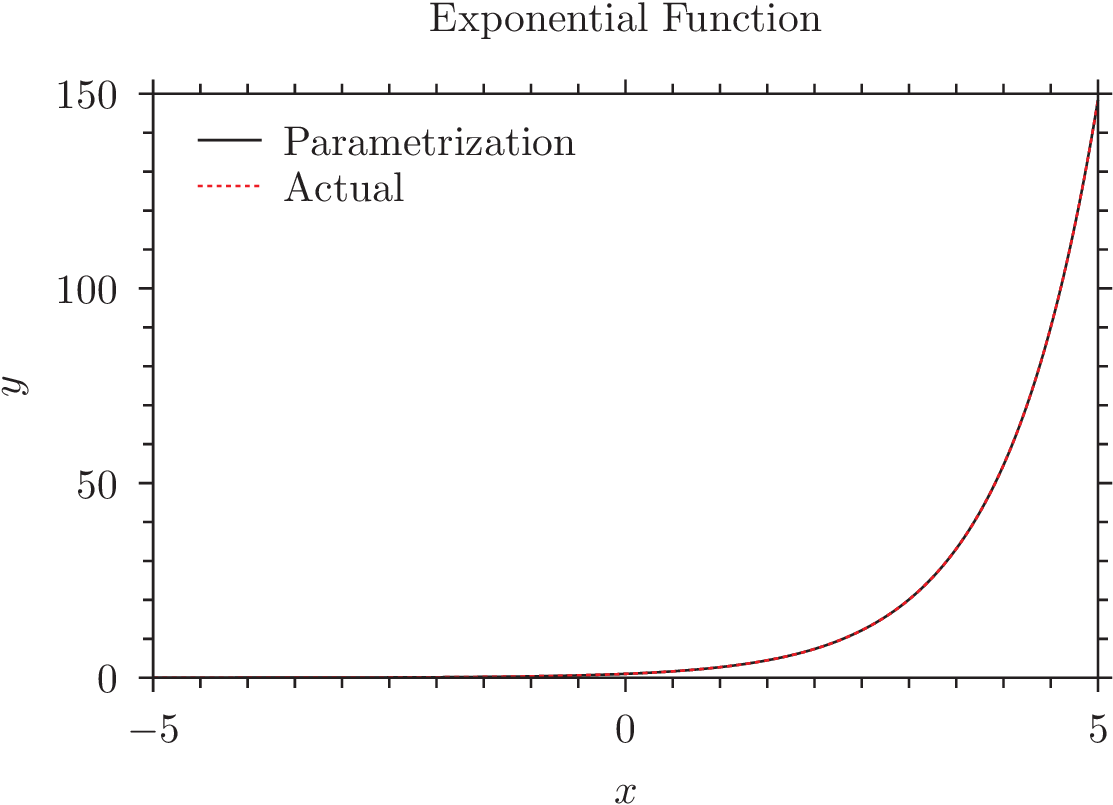
\includegraphics[width=0.4\textwidth]{out.png}
    \caption{Parametrization of the exponential function as presented in this report versus the actual implementation of the exponential function in the underlying C code that C\# calls into.}
    \label{fig:e}
\end{figure}

\end{document}
